% !TeX root = ../../thesis.tex
\chapter{Applications: Acetabular cup}\label{ch:cup}

\begin{shaded}
This chapter is based on prepared manuscript to be submitted to  \textit{IEEE Computing in Science \& Engineering}:\\
M. Barzegari, F. Perez-Boerema, G. Zavodszky, and L. Geris, ``High-performance computer simulation of biodegradation of optimized personalized implants; a case study of a patient-specific porous acetabular implant,'' will be submitted to \textit{IEEE Computing in Science \& Engineering}.
\end{shaded}

\section{Introduction}

Before we can take advantage of the interesting properties of metallic biodegradable implants, their biodegradation behavior needs to be evaluated and tuned for the target application. One example from orthopedics is tuning the degradation rate of implants to match the rate of bone formation. \textit{In silico} models can be beneficial in this regard as they can replace resource-consuming \textit{in vitro} or \textit{in vivo }experiments otherwise required. As a case study, in this work, we have developed a computational biodegradation model of a stiffness-optimized patient-specific porous acetabular implant.


\begin{figure}[h]
\centering
\medskip
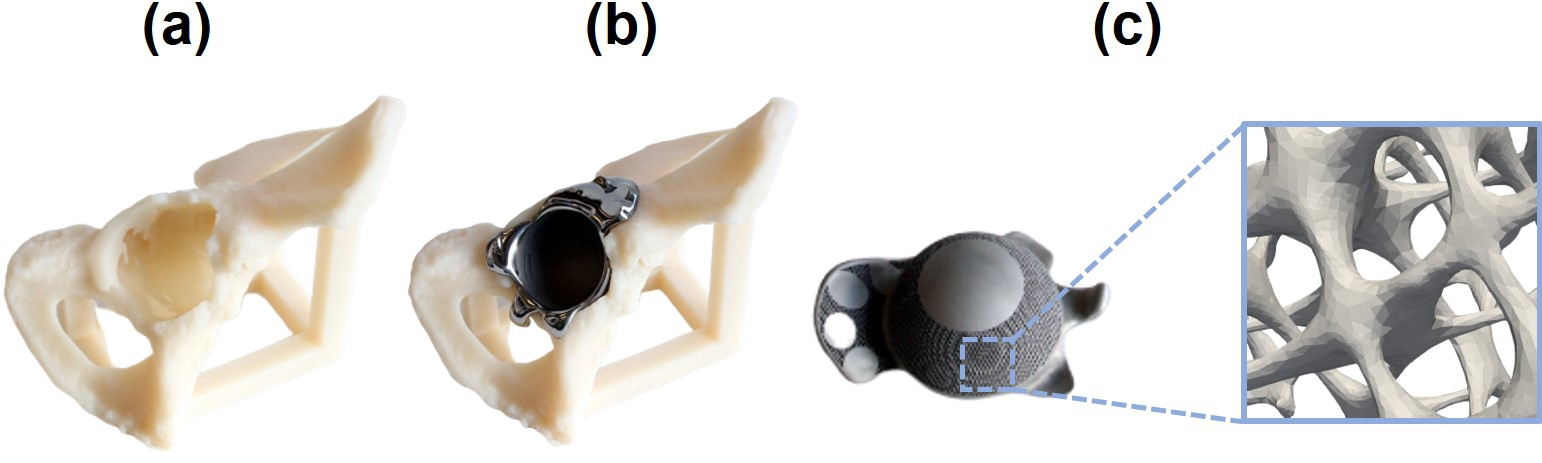
\includegraphics[width=\textwidth]{implant.jpg}
\caption[Application of the acetabular implant]{Demonstration of the application of a porous acetabular implant.} \label{fig:cup_implant}
\end{figure}

\section{Materials and Methods}

The computational model of the biodegradation process was constructed based on a mechanistic diffusion-reaction model that models the oxidation-reduction reactions occurring during the biodegradation process of metallic materials in simulated body fluid. The finite element method was used to solve the computational model \cite{Barzegari2021}. For building the lattice structure, the in-house developed open-source tool ASLI \cite{Perez-Boerema2022} was used to create a triply periodic minimal surface based infill for the acetabular implant based on the output of a patient-specific topology optimization. The resulting surface mesh, consisting of \num{5347924} faces, was subsequently converted to a volume mesh and embedded in a cubic container that was to act as the environment during the biodegradation simulations. The mesh was refined on the implant/environment interface to increase the numerical accuracy of the model, leading to a final mesh with \num{45870053} elements.

\begin{figure}[h]
\centering
\medskip
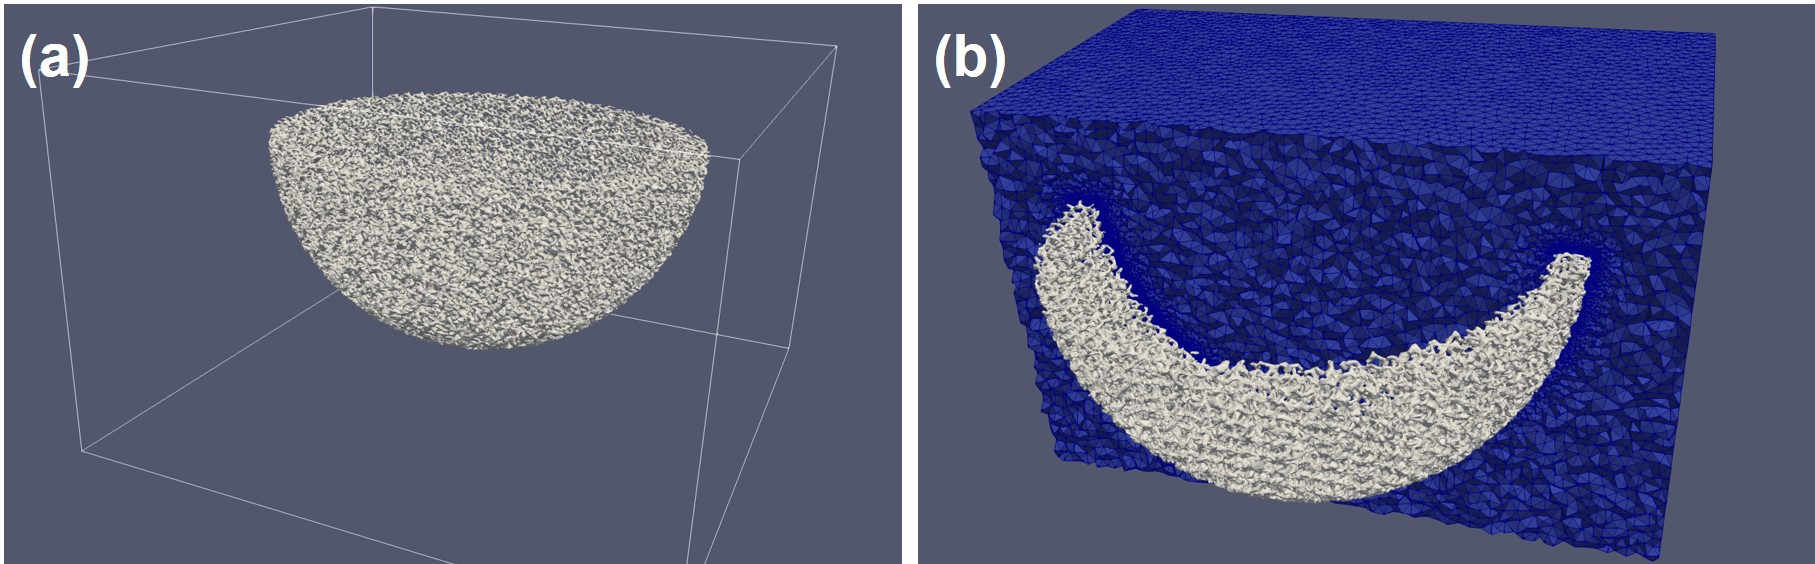
\includegraphics[width=\textwidth]{model.jpg}
\caption[Computational biodegradation model for the porous acetabular implant]{The computational model of the optimized acetabular implant embedded inside a cubic container.} \label{fig:cup_model}
\end{figure}

For dealing with a problem of this size and making the model capable of being scaled in large-scale computing systems, the model was implemented making use of the high-performance computing (HPC) techniques available in the FreeFEM language v4.10 and PETSc toolkit v3.16.1 \cite{Barzegari2022}. The simulation was carried out using 2,000 CPU cores with 16.5 TB of available memory. The results, with a total size of 148 GB, were visualized using a parallel ParaView server v5.9.1 running on 128 CPU cores. To obtain the scaling behavior of the model in an HPC environment scaling tests were performed by varying the number of employed CPU cores from 60 to \num{9000}.

\begin{figure}[h]
\centering
\medskip
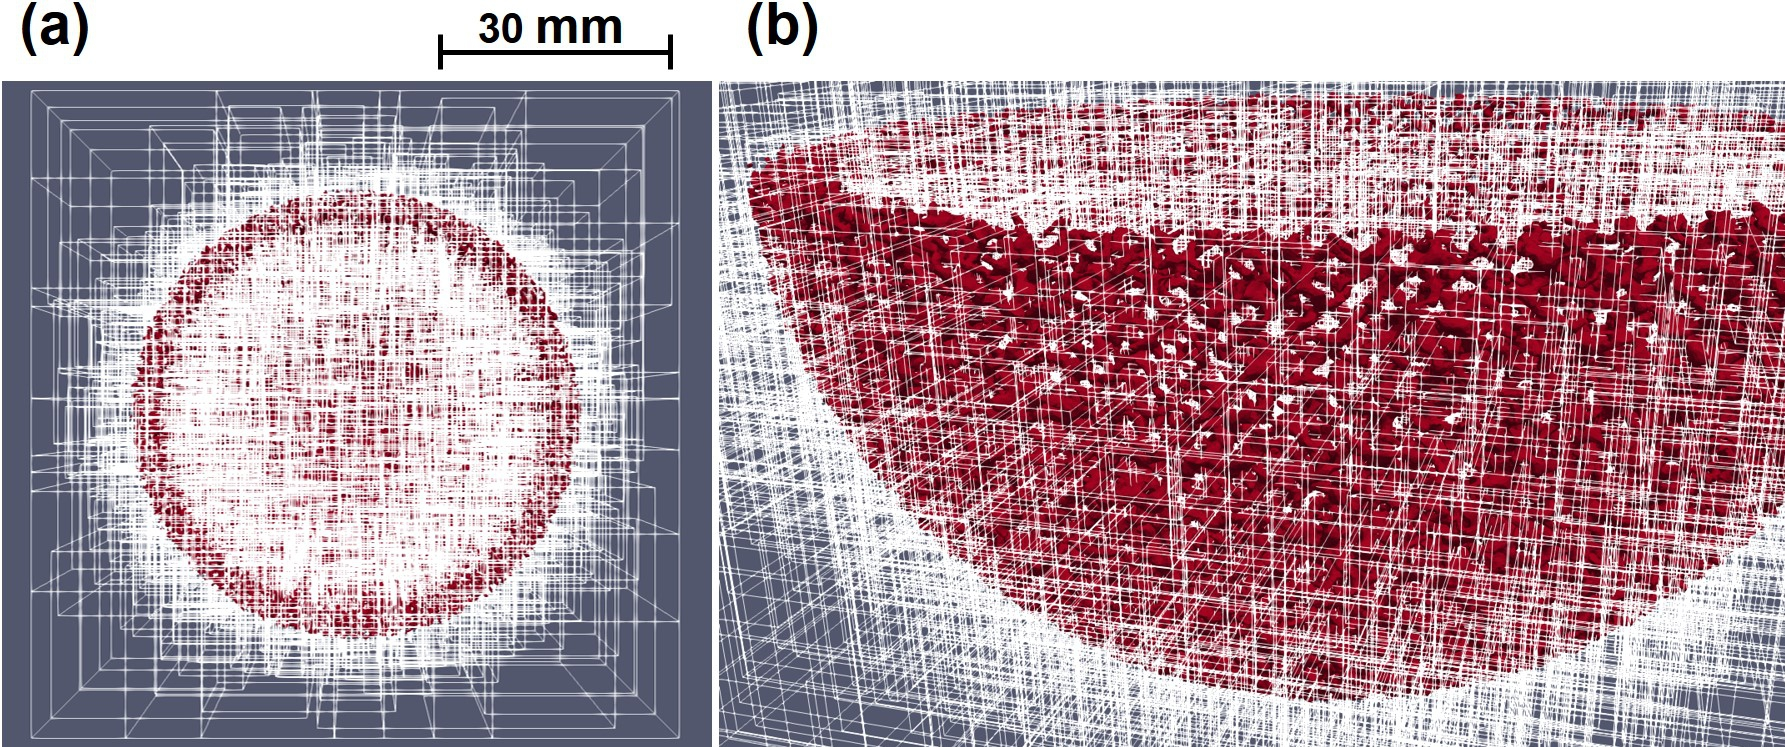
\includegraphics[width=\textwidth]{decomposition.jpg}
\caption[Mesh decomposition of the acetabular implant model]{Mesh decomposition of the computational biodegradation model to be distributed to available computing nodes.} \label{fig:cup_decomposition}
\end{figure}

\section{Results and Discussion}

The generated lattice structure of the implant, infilled by skeletal-gyroid unit cell type, is depicted in Fig. 1A. Biodegradation results show that the acetabular implant degrades faster in the region with higher porosity, i.e. the region with more exposed surface area to the environment (Fig. 1B). Loss of material over time was found to be in line with the values obtained in our previous study \cite{Barzegari2021}, showing that scaling the model in an HPC environment does not affect the quantitative predictions made by the model.  The scaling tests show that the optimal size for the distributed computing environment is \num{5000} CPU cores, above which no significant improvement in the execution time was observed.

\begin{figure}[h]
\centering
\medskip
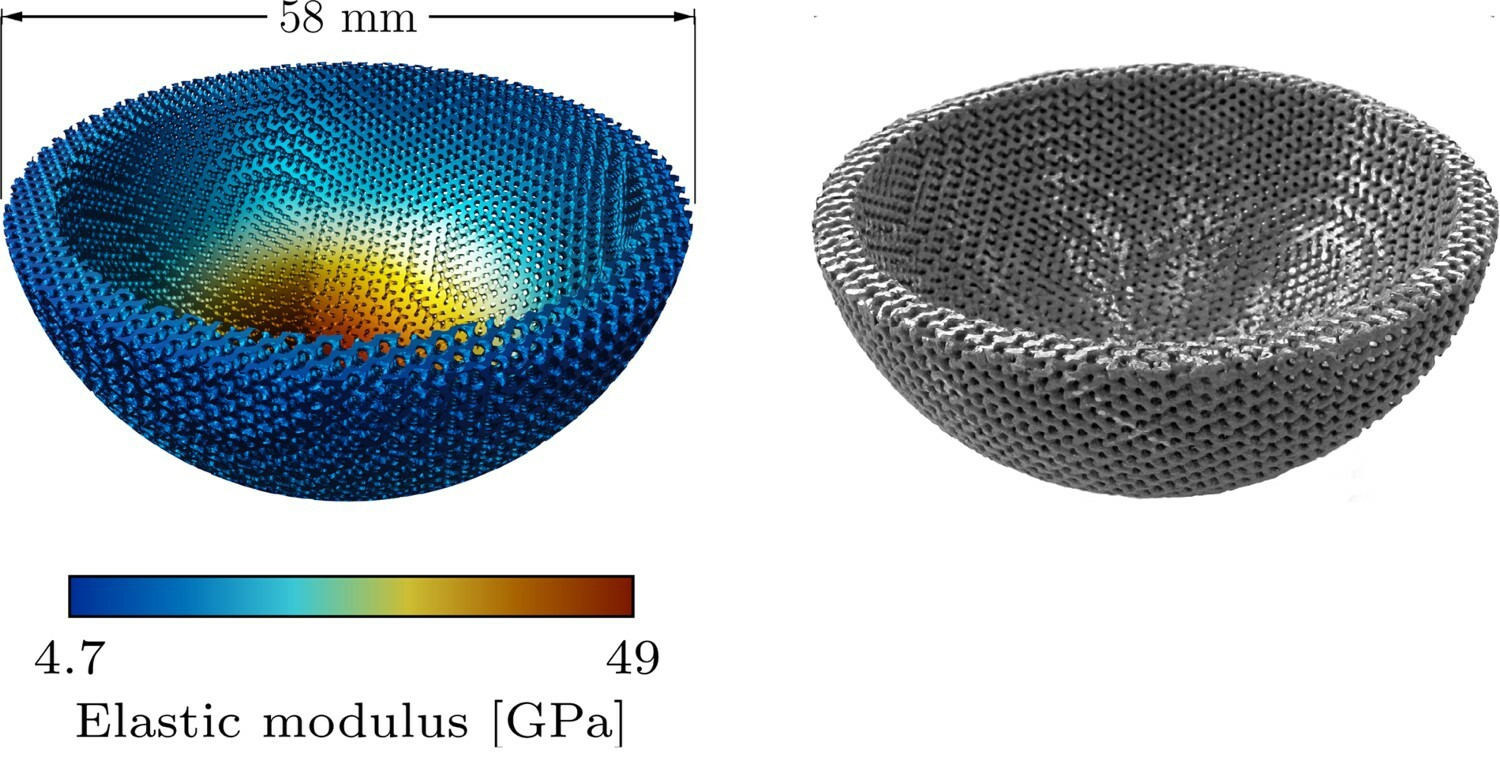
\includegraphics[width=\textwidth]{optimization.jpg}
\caption[Infilled acetabular implant]{Acetabular implant infilled by varying volume fraction to match a desired stiffness distribution.} \label{fig:cup_optimization}
\end{figure}

\begin{figure}[h]
\centering
\medskip
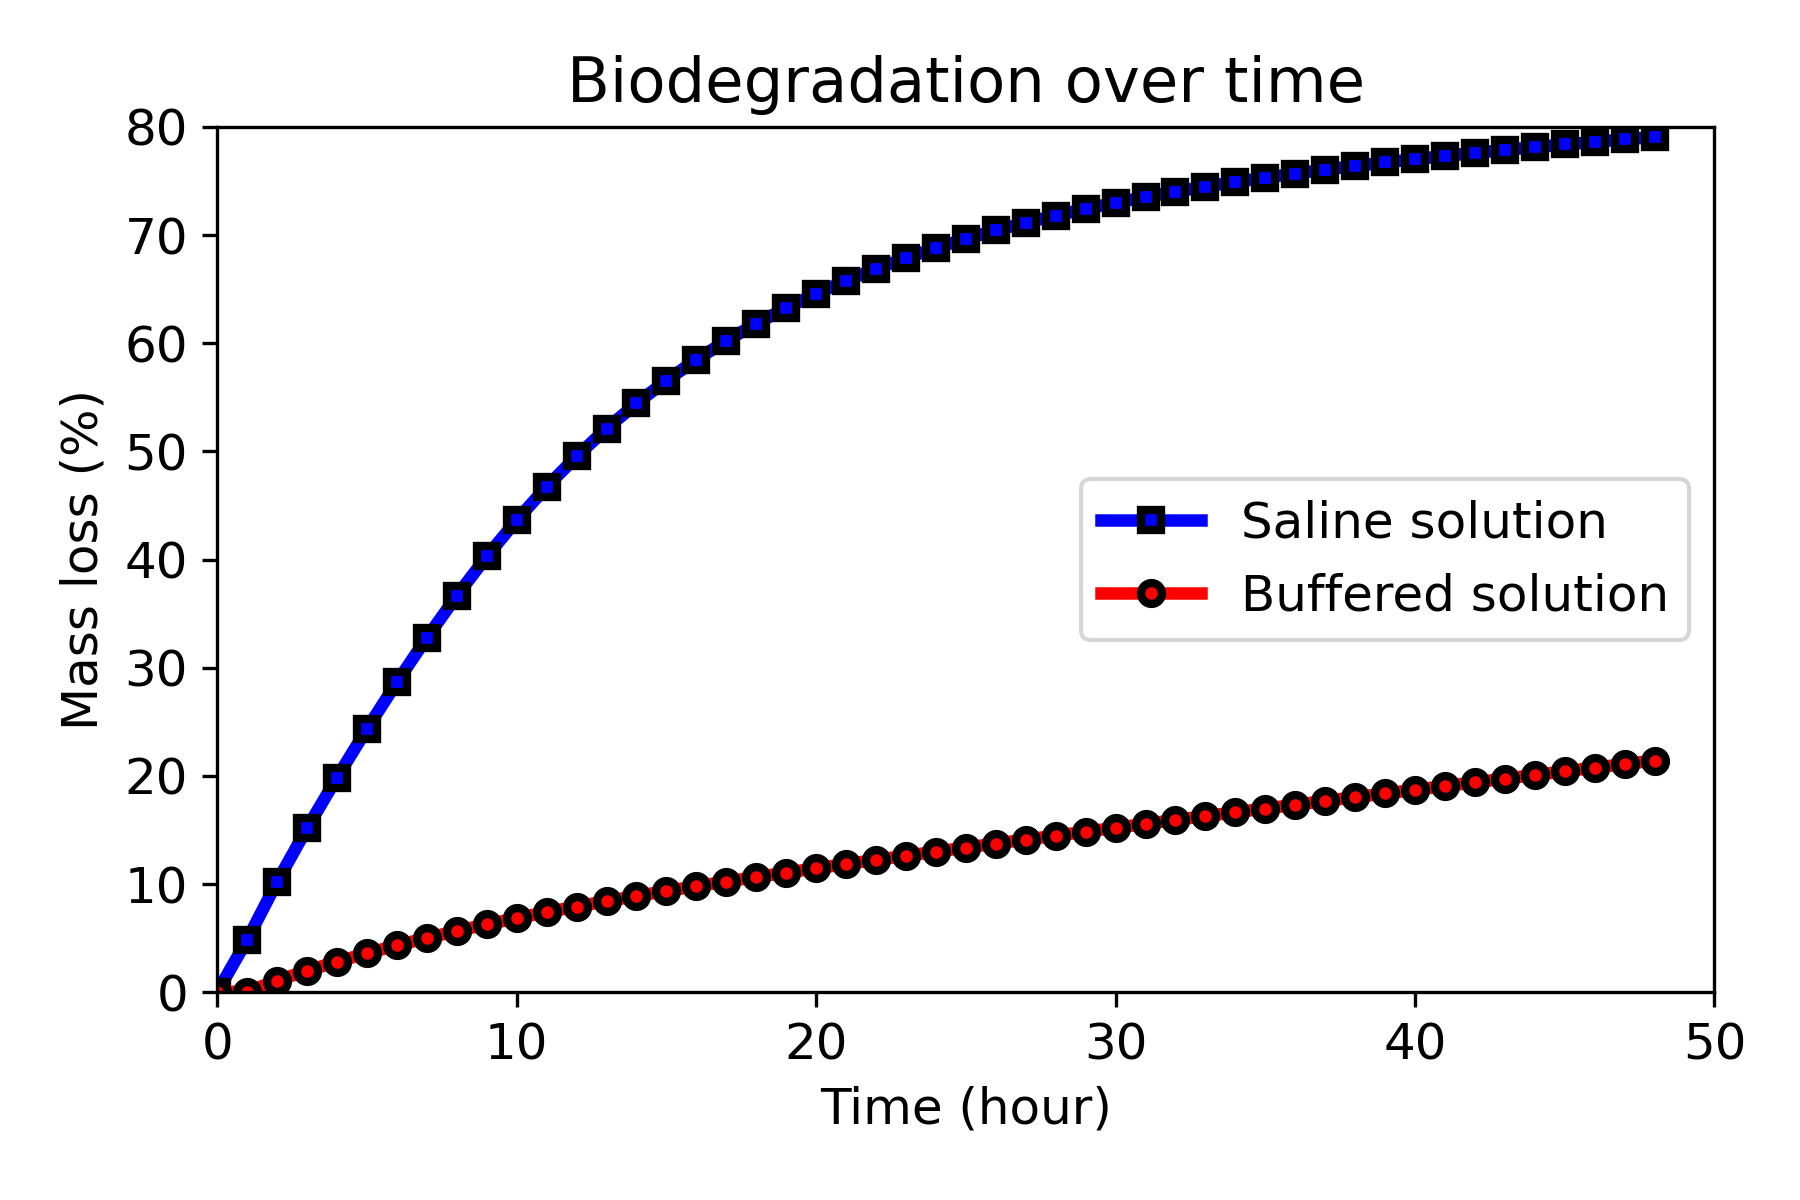
\includegraphics[width=0.9\textwidth]{degradation_rate.png}
\caption[Biodegradation rate for the acetabular implant]{Rate of mass loss during the biodegradation of the porous acetabular implant in saline and buffered solutions.} \label{fig:cup_degradation_rate}
\end{figure}

\begin{figure}[h]
\centering
\medskip
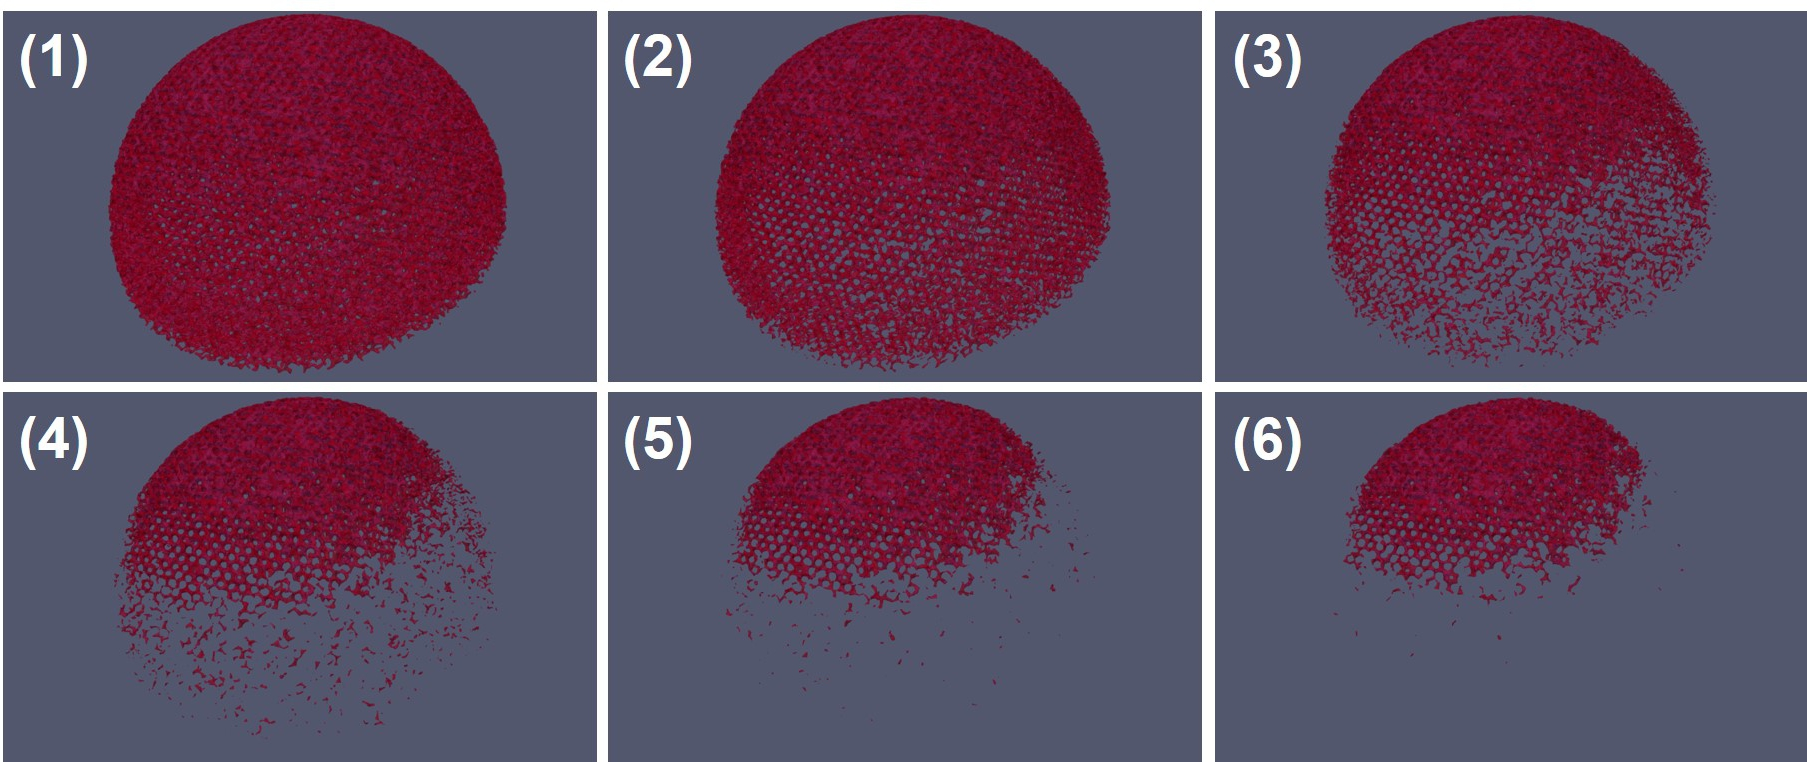
\includegraphics[width=\textwidth]{degradation_visual.jpg}
\caption[Visualization of the change of morphology of the acetabular implant]{Visualization of the change of morphology of the acetabular implant.} \label{fig:cup_degradation_visual}
\end{figure}

\begin{figure}[h]
\centering
\medskip
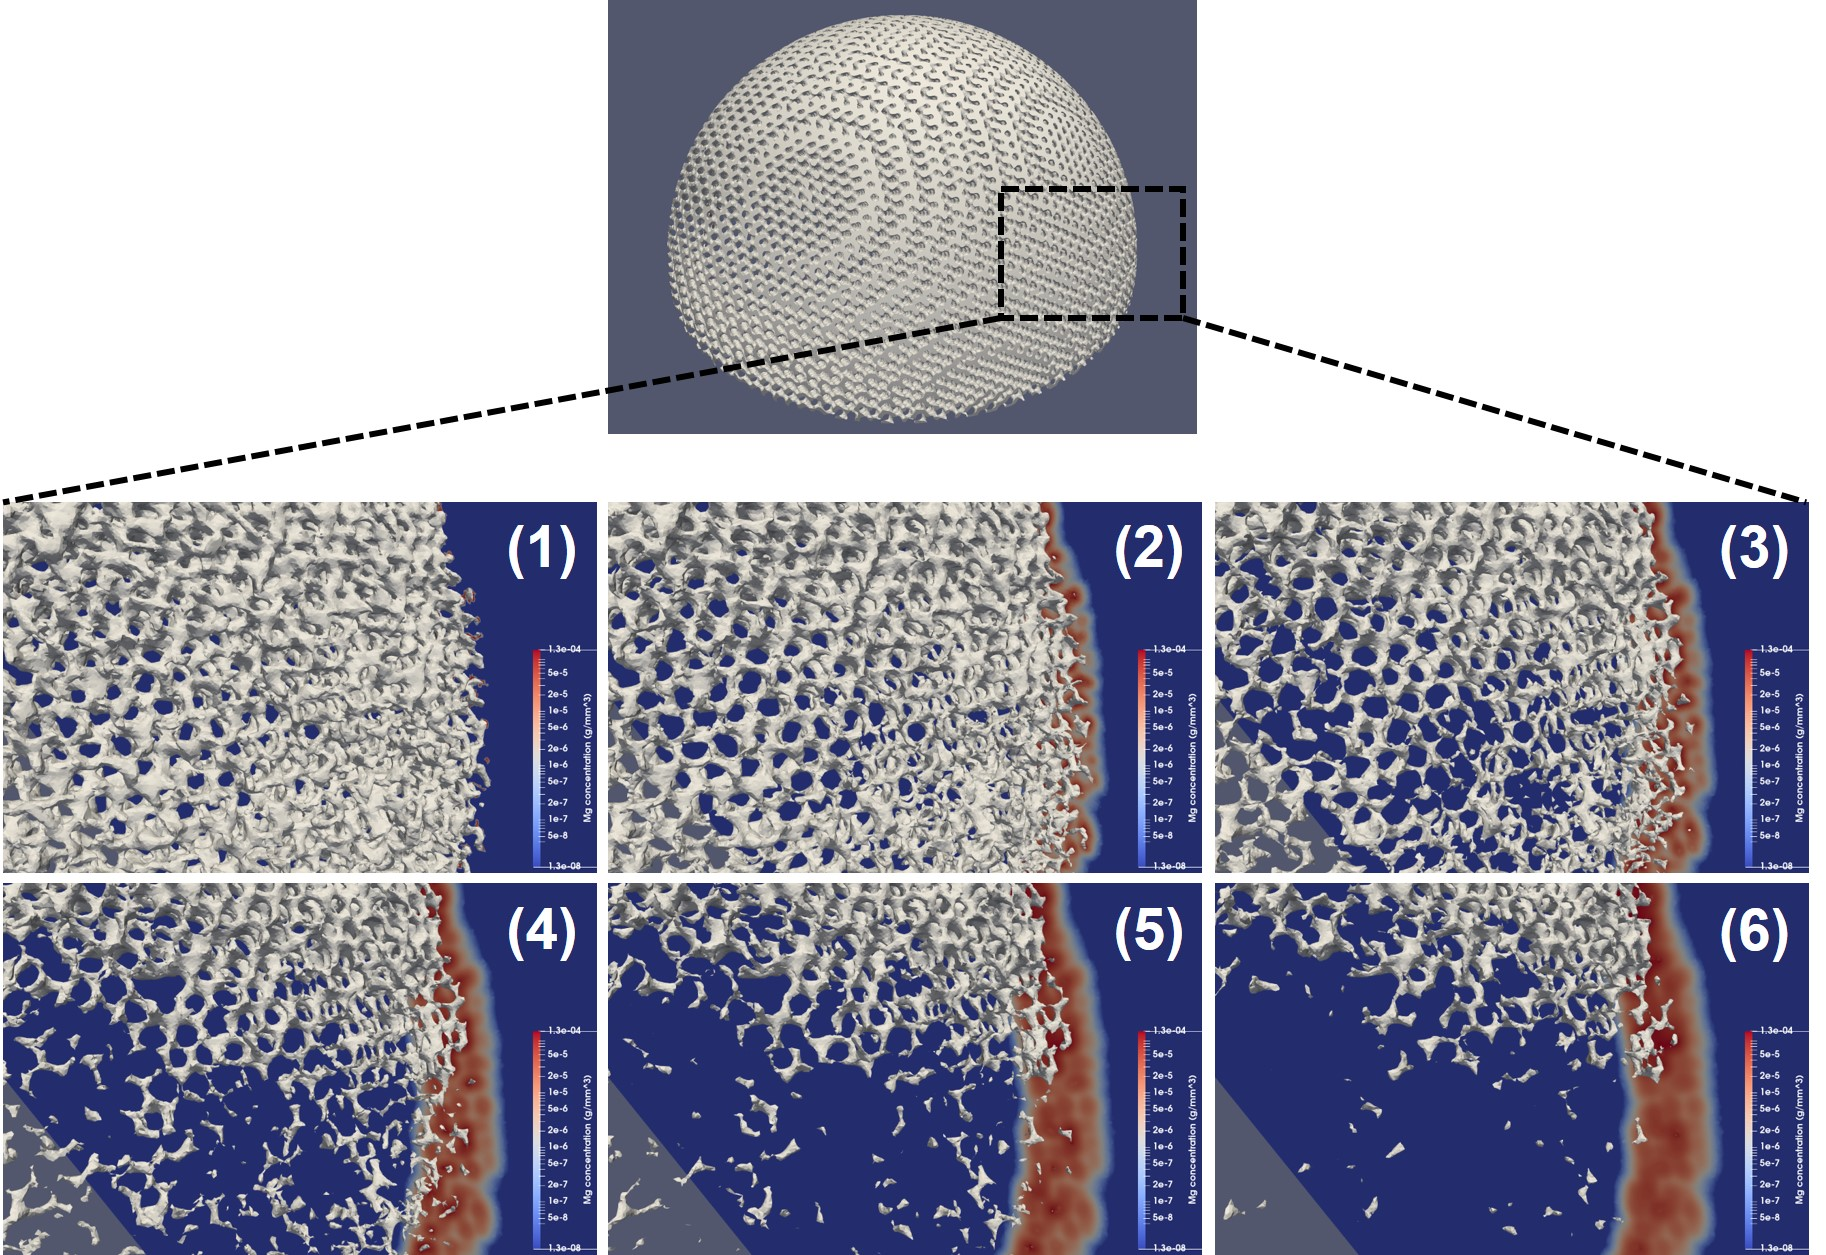
\includegraphics[width=\textwidth]{degradation_visual_close.jpg}
\caption[Visualization of the change of morphology of the acetabular implant]{Visualization of the change of morphology of the acetabular implant - zoom view.} \label{fig:cup_degradation_visual_close}
\end{figure}

\begin{figure}[h]
\centering
\medskip
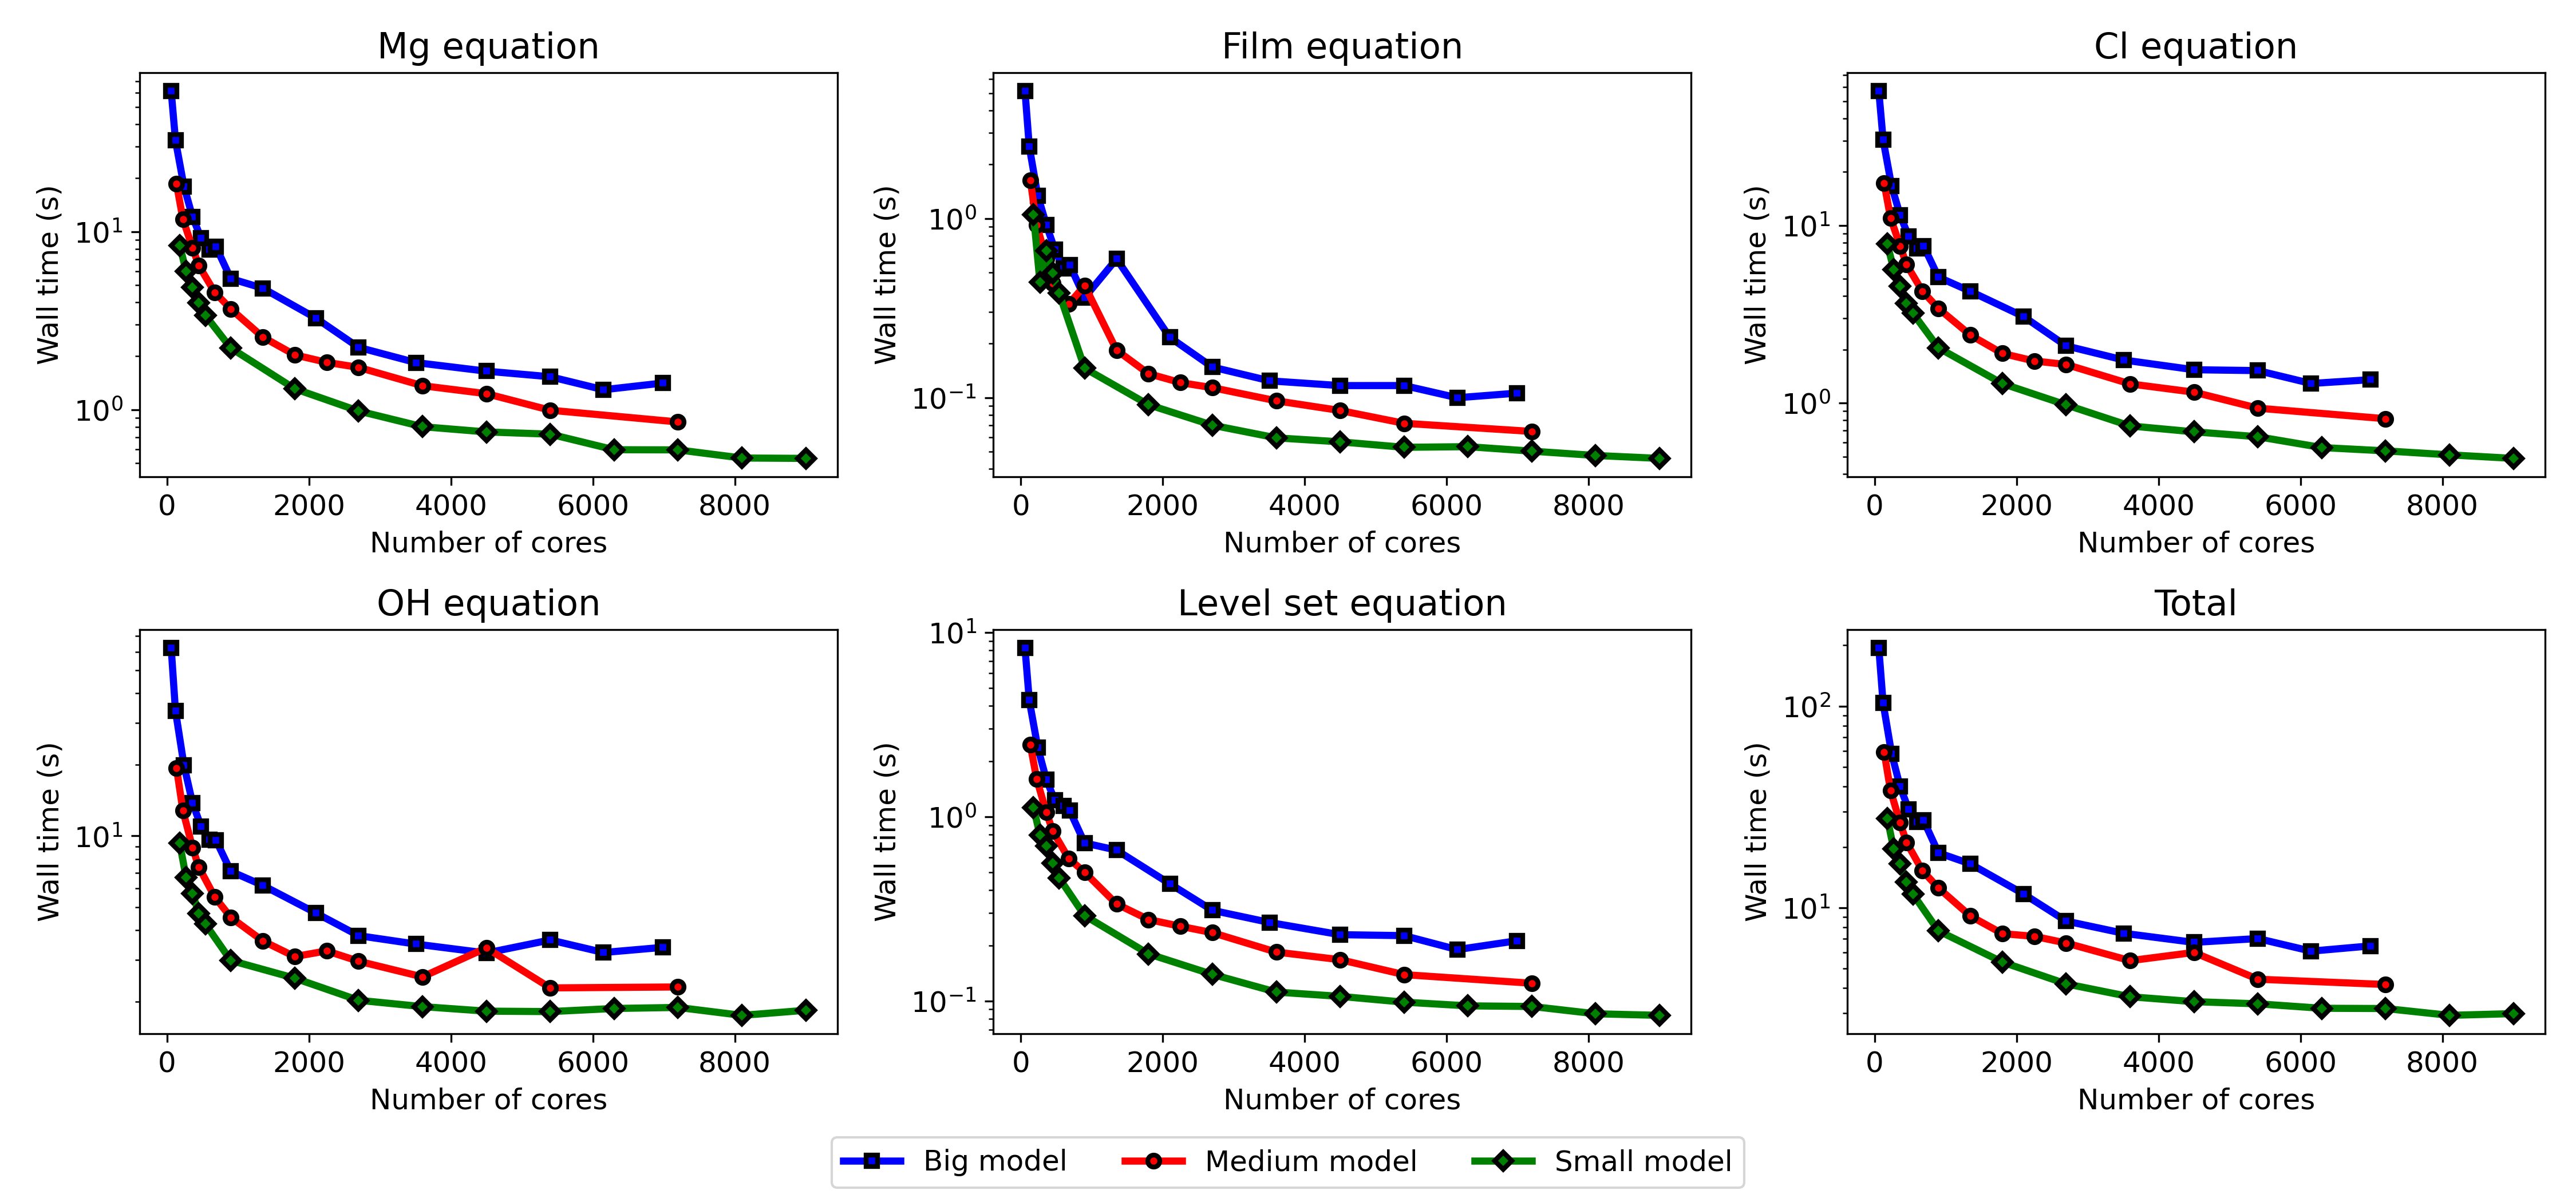
\includegraphics[width=\textwidth]{strong_scaling.png}
\caption[Strong scaling of individual components of the biodegradation model]{Strong scaling of individual components of the biodegradation model.} \label{fig:cup_strong_scaling}
\end{figure}


\begin{figure}[h]
\centering
\medskip
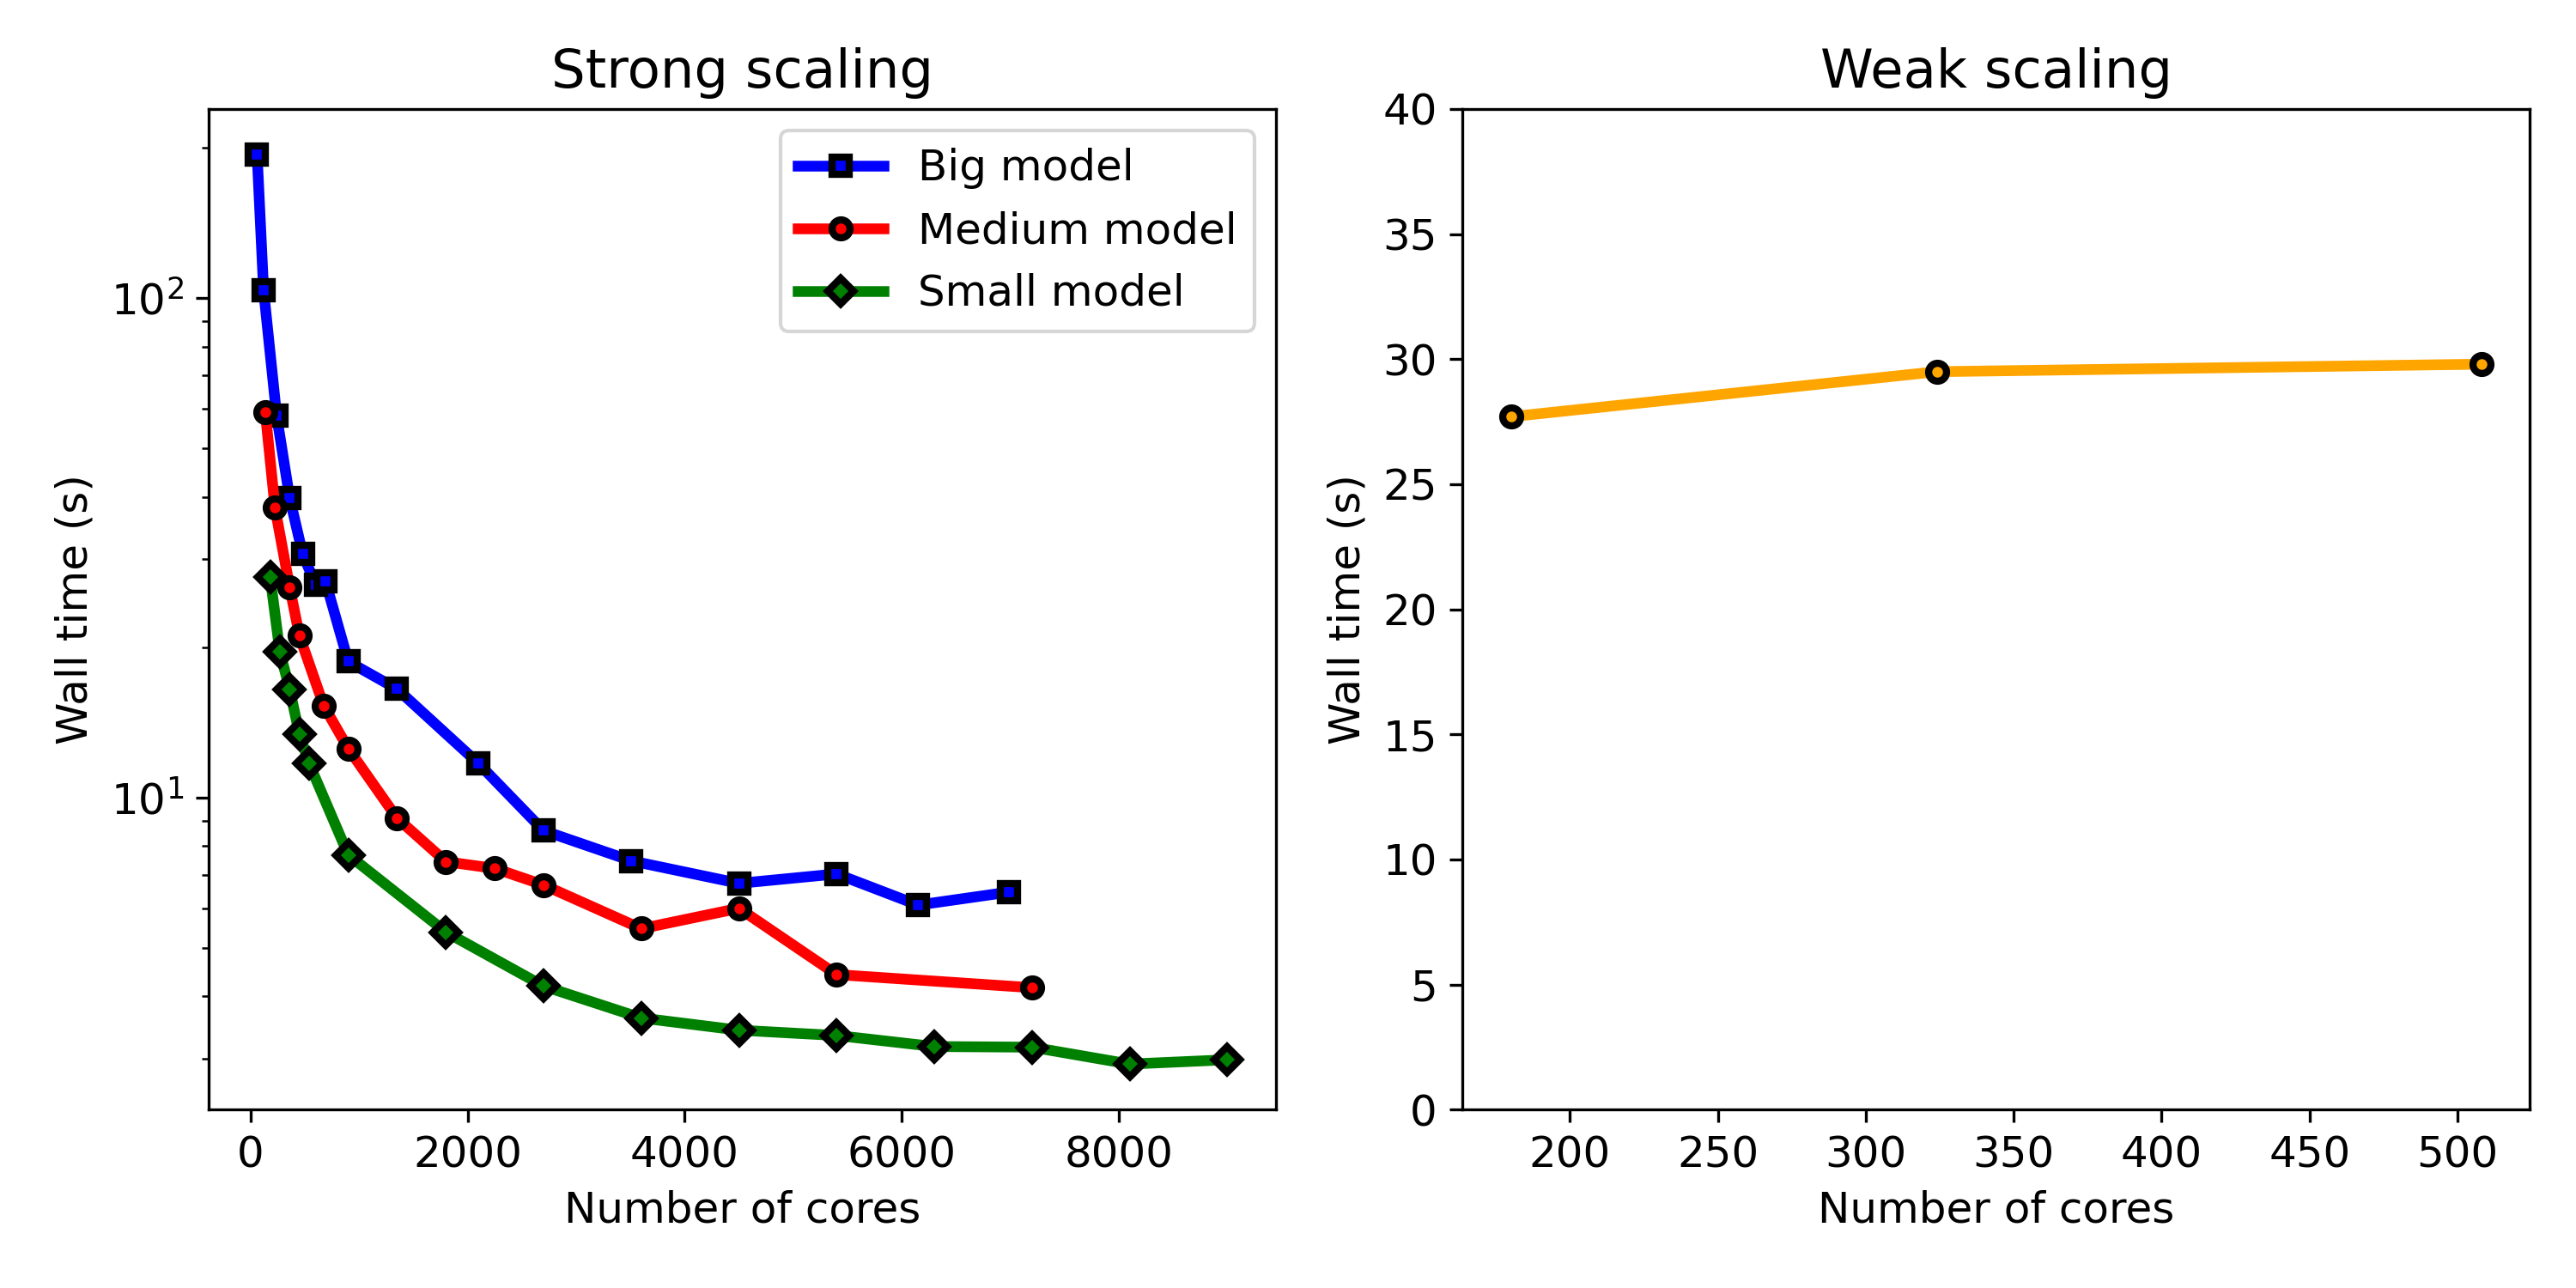
\includegraphics[width=\textwidth]{weak_strong.png}
\caption[Weak and strong scaling of of the acetabular implant model]{Weak and strong scaling of of the computational biodegradation model of the acetabular implant.} \label{fig:cup_weak_strong}
\end{figure}

\section{Conclusions}

In this work, taking advantage of HPC techniques to simulate a large-scale 3D model led to a computational model capable of predicting the biodegradation behavior of an acetabular implant in high resolution. Results demonstrate the potential of the model to act as a tool for assessing and tuning the biodegradation properties of orthopedic  implants regardless of shape or complexity.

\section{Acknowledgments}

Funded by Interreg VA Flanders - Netherlands, (2014TC16RFCB046, Prosperos) \& FWO-Vlaanderen (G085018N).

Dutch supercomputer - Snellius

UK supercomputer - ARCHER2


\begin{subappendices}

\section{Challenges in scaling the computational model to thousands of CPU cores}



\end{subappendices}


%%%%%%%%%%%%%%%%%%%%%%%%%%%%%%%%%%%%%%%%%%%%%%%%%%
% Keep the following \cleardoublepage at the end of this file, 
% otherwise \includeonly includes empty pages.
\cleardoublepage

